\documentclass[a4paper,11pt]{article}

% Packages for additional functionality
\usepackage[utf8]{inputenc} % For UTF-8 encoding
\usepackage{amsmath, amssymb} % For math symbols
\usepackage{hyperref} % For hyperlinks
\usepackage{listings} % For code blocks
\usepackage{xcolor} % For syntax highlighting in code
\usepackage{graphicx}
% Customize hyperlink colors
\hypersetup{
    colorlinks=true,
    linkcolor=blue,
    filecolor=magenta,      
    urlcolor=cyan,
}

% Set the default font style
\renewcommand{\familydefault}{\sfdefault}

% Code block style
\lstset{
    basicstyle=\ttfamily\small,
    backgroundcolor=\color{lightgray},
    frame=single,
    breaklines=true,
    postbreak=\mbox{\textcolor{red}{$\hookrightarrow$}\space},
}

% Document starts
\begin{document}

% Title and Author Information
\title{Quickstart guide for UniNuvola usage}
\author{Marco Pezzella}
\date{18/10/2024}

\maketitle

%\tableofcontents
%\newpage
\section{Introduction}

Welcome to this quickstart guide for using UniNuvola. This is not a comprehensive manual—one will be made available soon—but it provides the information required to start using the prototype server.

\section{Accessing the server}

You can access UniNuvola via any web browser through the website \href{https://what-if.xkcd.com/1/}{https://what-if.xkcd.com/1/}. If it is your first time accessing the server, you will be redirected to a small form page, where you can request access. Access will be granted once one of the operators approves your request. When accepted, or if you already have an account, you will be redirected to the UniNuvola Vault login page. After selecting the LDAP option in the drop-down menu, you can enter your login details. These are the same as those you use to access the University email.

\section{Selection of the Image and resources}

\textbf{Note:} This section will undergo further modifications within the next month, and the quickstart will be updated accordingly.

After a successful login, you will be directed to the resource selection page. The first section to complete is the image selection. This part needs to be filled in by the user. Images can be selected from those available in UniNuvola (see table \ref{tab:images}) or from your own customised version on Dockerhub. The tags \textit{latest} and \textit{deployed} are available.\\

\begin{table}[]
\caption{List of the official images in UniNuvola}
\label{tab:images}
\centering
\begin{tabular}{|c|c|}
\hline
Base & Row 1, Col 2 \\ \hline
Engineering & Row 2, Col 2 \\ \hline
Conda & Row 3, Col 2 \\ \hline
Chemistry & Row 4, Col 2 \\ \hline
Quantum Computing & Row 5, Col 2 \\ \hline
Genomics & Row 6, Col 2 \\ \hline
Hydraulics & Row 7, Col 2 \\ \hline
Tensorflow & Row 8, Col 2 \\ \hline
Pytorch & Row 9, Col 2 \\ \hline
Pytorch-GPU & Row 10, Col 2 \\ \hline
\end{tabular}
\end{table}


The image name will appear as: 
\begin{lstlisting}[language=bash] 
Shall we play a game
\end{lstlisting}

In the next drop-down menus, you will choose the number of CPUs required (N1, N2, N3), the amount of RAM required (R1, R2, R3), and, if you require GPUs, the number of them (G1, G2, G3). At the moment,  a S1 gigabyte of persistent storage is available for each user.\\

As per the disclaimer, remember: \textbf{UniNuvola is a prototype. We provide computational power and storage, but data are not backed up. Be careful with your data!} \\

\section{Inside UniNuvola}
The main page of UniNuvola appears as depicted in Figure \ref{fig:uninuvola_main_page}. The top bar allows some management actions and some customisation of the user interface. Most importantly, inside the file men, you can find the disconnect and  the control hub options. The former allows to connect and disconnect from Jupyter (be aware that you will disconnect from the Hub page, but the pod will continue run up to XX from inactivity), the later option allows to kill the running image and it allows the user to load a new image. \\ 

the left side of the menu allows the management of the local files and, in future, to mount filesystems containing large size program files and libraries. The four most upper options allow the user in order to: open new launchers tabs, create new directories, upload files, and refresh the browser. \\

The orange square includes all Python and R toolkits. The top part includes all the environments notebooks in the image, the bottom part instead the relative consoles. The top right part, the purple square, contains the Xpra notebook, that allows the usage of programs requiring a graphical interface.  \\

in the last line, the first element, circled in green, allows the user to use a terminal. All terminals will start with the sh/bash terminal depending on the image. The elements circled in blue are the text editors in the Hub,  in the case of the figure a general text editor, a Markdown and a Python file editor. \\ 


\begin{figure}[!ht]
    \centering
    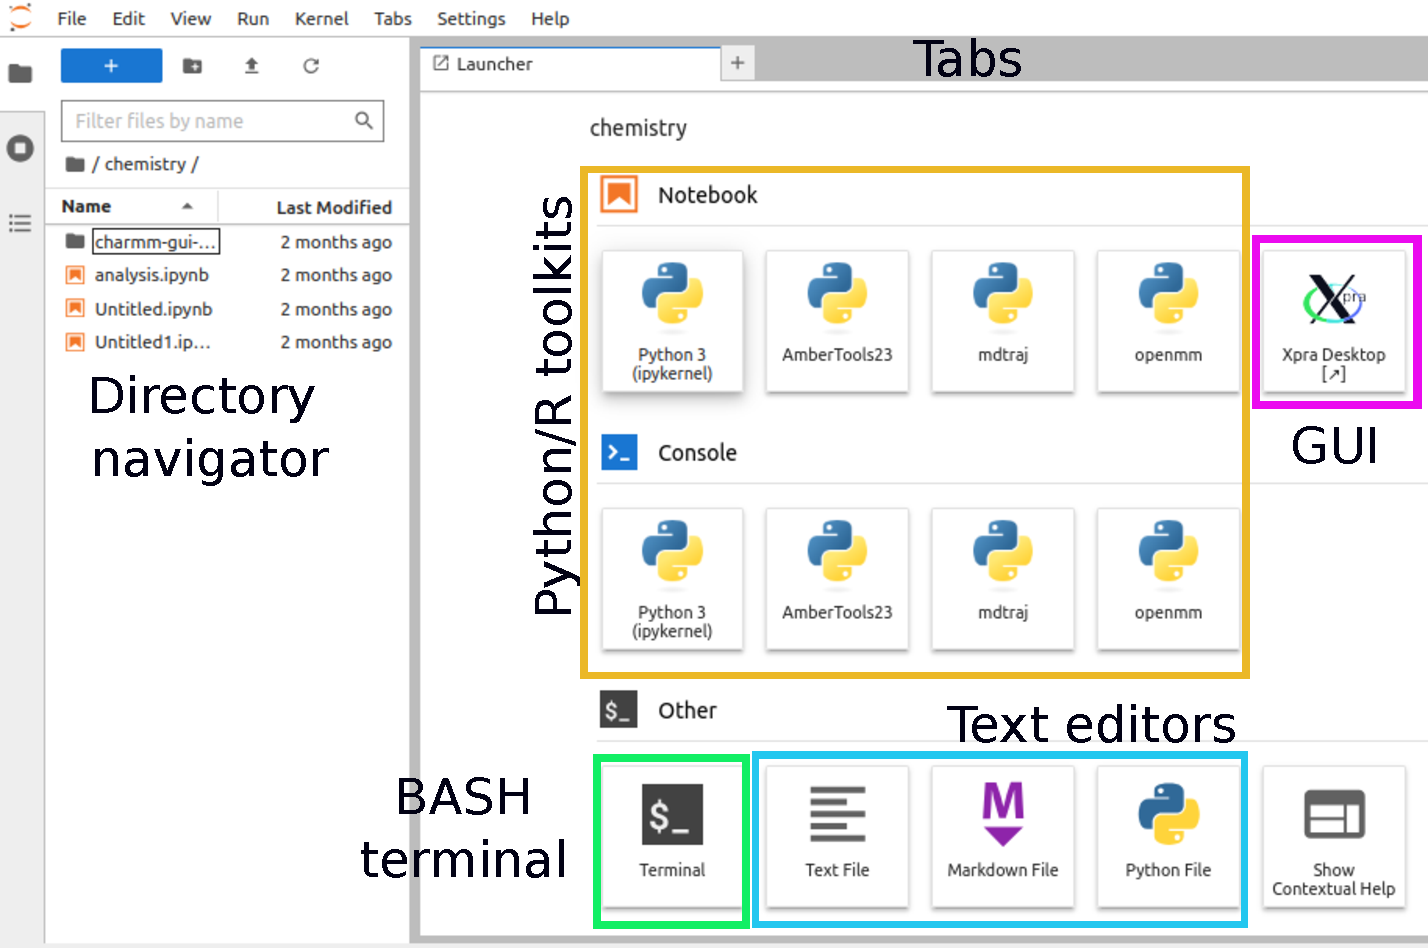
\includegraphics[width=0.8\linewidth]{uninuvola.pdf}
    \caption{Caption}
    \label{fig:uninuvola_main_page}
\end{figure}

\end{document}
